\chapter{Specification and system design}
\label{spec}
\section{Data collection}
The quantity and the quality of training data is crucial to all computer vision 
projects. However, for this task there was no luxury of using an existing 
dataset with the required level of detail in labels that would also be 
affordable.

A decision was made to collect own data for this project from a social network 
that makes it easy to associate user profiles with photos of themselves with 
locations accurate to city-level. Popular social networks such as Facebook 
would be ideal for this, however it is not possible to obtain a list of 
profiles from a hand-picked location due to Facebook API constraints. 
Moreover, it is clearly stated in Facebook's Terms and Conditions that any way 
to circumvent these constraints would still count as a violation.


\subsection{Tinder}
Tinder is a mobile dating application that shows profiles closest to the 
user's GPS location. There have been numerous third-party Tinder utilities on 
the Web that reverse-engineered Tinder's simple and unobfuscated HTTP API that 
makes it possible to create a fully-featured Tinder client yourself.

The API has support for various actions such as liking and messaging users, 
but for the purposes of this project, the only relevant actions to us are 
authentication, setting own location using latitude and longitude coordinates 
and fetching nearby users.


\subsection{Authentication}
Tinder profiles are created using Facebook OAuth. When the application is 
opened for the first time by a non-registered user, they will be prompted to 
login using Facebook OAuth which gives Tinder access to the user's full name, 
age, pictures and other details.

A user profile was created specifically for this project using the original 
Tinder mobile application on an Android phone. 

A Google Chrome extention was written in order to obtain an authentication 
token for the Tinder app on Facebook which must be sent with every request to 
the Tinder API. The extension adds a button to the Google Chrome toolbar which 
opens a static webpage that sends a request back to the extension to open the 
following URL:
\begin{logs}
https://www.facebook.com/v2.0/dialog/oauth
    ?response_type=token
    &display=popup
    &api_key=464891386855067
    &redirect_uri=fbconnect%3A%2F%2Fsuccess
    &scope=user_about_me%2Cuser_activities%2Cuser_education_history%2Cuser_location%2Cuser_photos%2Cuser_relationship_details%2Cuser_status'
\end{logs}
where \texttt{api\_key} specifies the Tinder application ID on Facebook and 
\texttt{scope} lists the type of information Tinder will gain access to. This 
page asks the user to sign in with their Facebook credentials and, if 
successful, will save a cookie that will be sent along with the next request:

\begin{logs}
POST https://www.facebook.com/v2.0/dialog/oauth/confirm

{
  "app_id: "464891386855067",
  "ttstamp: "2658170904850115701205011500",
  "redirect_uri": "fbconnect://success",
  "return_format": "access_token",
  "from_post": 1,
  "display": "popup",
  "gdp_version": 4,
  "sheet_name": "initial",
  "__CONFIRM__": 1
}
\end{logs}
The response to this will contain an access token that will be used to 
interact with the Tinder API. It can be extracted using 
\begin{logs}
    access_token=([\w_]+)&
\end{logs} 
as a regular expression. It will be referred to as \texttt{<fb\_token>} from 
this point on.

Before we can use it to authenticate with Tinder the Facebook user ID must 
also be obtained by accessing 
\texttt{https://graph.facebook.com/me?access\_token=\textbf{<access\_token>}}.
The response to this request is a JSON object which contains the Facebook user 
ID under the property \texttt{id}, which will be known as 
\texttt{<fb\_user\_id>}.

Now that we have the Facebook user ID and User Access Token it is possible to 
authenticate with Tinder as follows:

\begin{logs}
POST https://api.gotinder.com/auth

{
    "facebook_token": <access_token>, 
    "facebook_id": <fb_user_id>
}
\end{logs}

The response to this request is a JSON object containing Tinder's own 
authentication token and user ID. Tinder's authentication token is saved in 
memory and sent as an HTTP header \texttt{X-Auth-Token} with every request 
after authentication.


\subsection{Updating location}
Updating the location of the user profile is simply a matter of sending the 
new latitude and longitude values via a \texttt{POST} request as follows:
\begin{logs}
POST https://api.gotinder.com/user/ping

{
    "lat": <new_latitude>
    "lon": <new_longitude>
}
\end{logs}
This is performed after authentication with latitude and longitude as 
specified in the data collection job (see \ref{spec:data:jobs}).

The limitation with this method of changing own location is that it is not 
possible to change the location too frequently if the distance between the new 
and the old locations is too large to be travelled in the amount of time 
passed.

\subsection{Fetching profiles and images}
User profiles are internally referred to as \textit{recommendations} by Tinder and 
can be retrieved using the following \texttt{POST} request:
\begin{logs}
POST https://api.gotinder.com/user/recs

{
    "limit": <job_limit>
}
\end{logs}
The \texttt{limit} option refers to the maximum number of users that can be 
fetched at once. The value for \texttt{limit} comes from the corresponding 
data collection job (\ref{spec:data:jobs}).

The JSON response contains a property called \texttt{results} which is an 
array of profiles (\texttt{Array<Profile>}). Every profile contains properties 
as specified in Table \ref{table:profile-properties}.
\begin{table}
    \begin{center}
        \begin{tabular}{| l | c | c |}
            \hline
            Property       & Data type               & Example \\ \hline
            distance\_mi   & integer                 & 2 \\ \hline
            \_id           & char[24]                & 518d666a2a00df0e490000b9 \\ \hline
            birth\_date    & RFC 3339 date and time  & 1986-05-17T00:00:00.000Z \\ \hline
            gender         & integer                 & 1 \\ \hline
            name           & string                  & Elen \\ \hline
            photos         & Array<Photo>            & N/A \\ \hline
        \end{tabular}
    \end{center}
    \caption{Properties of a Tinder profile as retrieved using the API. 
        Properties not used in this project have been stripped out.}
    \label{table:profile-properties}
\end{table}
% "url": "http://images.gotinder.com/518d666a2a00df0e490000b9/fea4f480-7ce0-4143-a310-a03c2b2cdbc6.jpg"
Table \ref{table:photo-properties} shows the relevant properties of profile 
photos.

\begin{table}
    \begin{center}
        \begin{tabular}{| l | c | c |}
            \hline
            Property       & Data type               & Example \\ \hline
            \_id           & UUID                    & fea4f480-7ce0-4143-a310-a03c2b2cdbc6 \\ \hline
            fileName       & string                  & fea4f480-7ce0-4143-a310-a03c2b2cdbc6.jpg \\ \hline
            extension      & string                  & jpg \\ \hline
            url            & URL                     & http://images.gotinder.com/<profile\_id>/<image\_id>.jpg \\ \hline
        \end{tabular}
    \end{center}
    \caption{Properties of a Tinder image as retrieved using the API. 
        Properties not used in this project have been stripped out.}
    \label{table:photo-properties}
\end{table}
The request above is performed every \texttt{<delay>} seconds, the value for 
which is specified as part of a data collection job (see \ref{spec:data:jobs}).

\subsection{Tinder job manager}
\label{spec:data:jobs}
Tool to manage Tinder jobs.
Images of people need to be collected from a number of different locations 
around the world. Specifying the coordinates of each location using latitude 
and longitude values proved to be cumbersome in the beginning which is why a 
special and user-friendly tool was written to manage data collection from the 
command line.

This tool resides in the \texttt{tinder-gather} project in the \texttt{tools} 
directory. Usage and help will be displayed in the terminal if ran with these 
arguments:
\begin{logs}
./jobs.js tjob post
\end{logs}

This command expects three arguments: location, limit and delay. Location is 
just a city name whose location is hard-coded inside the script and can be 
easily extended. This argument is required. Limit refers to the maximum number 
of profiles to fetch from Tinder at once and delay specifies how frequently 
they will be fetched.

This tool is also used to manage face and landmark detection jobs which will 
be described in detail in Section \ref{spec:fd}. 


\subsection{Technical details}
This entire data collection suite is written in JavaScript for Node.js and can 
be found in the \texttt{tinder-gather} directory. The Google Chrome extension 
is also written in JavaScript and the name of its project directory is 
\texttt{tinder-gather-connect}.

\texttt{tinder-gather} is a web application which was made possible using the 
Express.js web application framework. It provides a RESTful HTTP API to manage 
data collection jobs as well as a few debugging pages for viewing face 
detection results.

%Specifically, it uses a single HTTP resource (\texttt{/job}) and four 
%different HTTP verbs to control its ...

Profiles and user images found using a modified version of the Tinder.js 
library that implements the Tinder API are stored on disk in the 
\texttt{tinder-gather/gather-images} directory. The metadata for both profiles 
and images is stored in a PostreSQL database using an ORM library called 
Sequelize, which means it can be easily swapped for an alternative SQL 
database.

Figure \ref{fig:spec:erd_basic} shows the ER diagram for the data collection-
specific part of the database as well as entity \texttt{Detection Job} which 
will be covered in Section \ref{spec:fd}.

The names in parentheses correspond to the actual, case-sensitive table names 
in the PostgreSQL database. 
\begin{figure}[t]
  \centering
  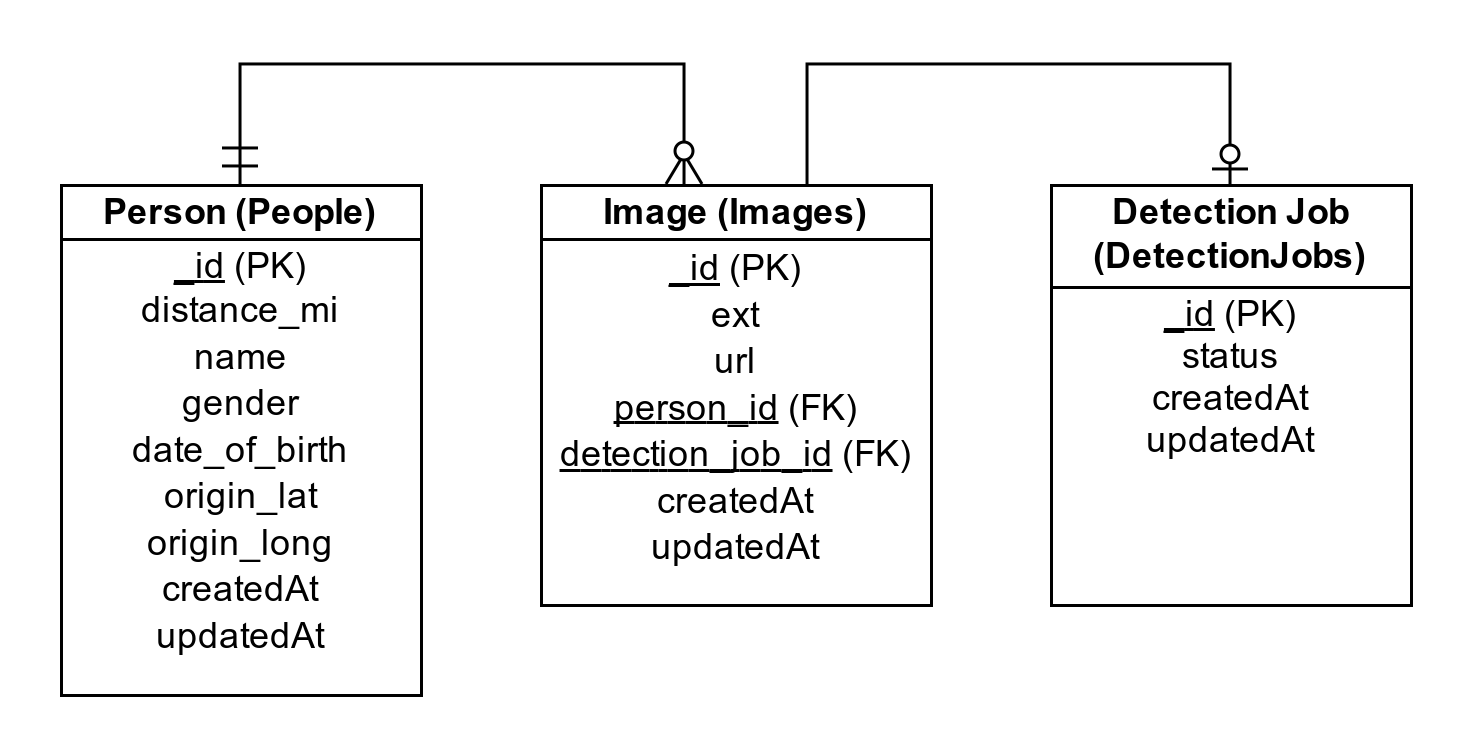
\includegraphics[width=\textwidth]{figures/spec/erd_basic}
  \caption{Entity-relation diagram for tables used by the data collection 
  application \texttt{tinder-gather}. }
  \label{fig:spec:erd_basic}
\end{figure}

\begin{table}[t]
    \begin{center}
        \begin{tabular}{| c | c | c |}
            \hline
            Attribute       & Data type              & Other \\ \hline
            \multicolumn{3}{|c|}{Person (People)} \\ \hline
            \_id           & character(24)            & not null   \\ \hline
            distance\_mi   & integer                  &            \\ \hline
            name          & character varying(255)   &            \\ \hline
            gender        & integer                  &            \\ \hline
            date\_of\_birth & integer                  &            \\ \hline
            origin\_lat    & double precision         &            \\ \hline
            origin\_long   & double precision         &            \\ \hline

            \multicolumn{3}{|c|}{Image (Images)} \\ \hline
            \_id              & character(36)            & not null   \\ \hline
            ext              & character varying(4)     &            \\ \hline
            url              & character varying(255)   &            \\ \hline
            person\_id        & character(24)            &            \\ \hline
            detection\_job\_id & integer                  &            \\ \hline

            \multicolumn{3}{|c|}{Detection Job (DetectionJobs)} \\ \hline
            \_id      & integer                     & not null, auto-increment \\ \hline
            status    & enum{started, finished}      &         \\ \hline

            \multicolumn{3}{|c|}{Common among all tables} \\ \hline
            createdAt & timestamp with time zone     & not null  \\ \hline
            updatedAt & timestamp with time zone     & not null  \\ \hline
        \end{tabular}
    \end{center}
    \caption{Attribute data types of entities introduced in Figure 
    \ref{fig:spec:erd_basic}}
    \label{table:spec:erd_basic_dt}
\end{table}

\section{Face and landmark detection}
\label{spec:fd}
Before the collected images from different parts of the world could be used to
learn how to determine the location of a person from a single picture of 
their face they must first be heavily filtered as many Tinder users upload
very low-quality pictures or even pictures of pets and inanimate objects.

A face detector is an ideal method of filtering out non-face images as well as
heavily edited or poor quality face images. 
...
\section{Preprocessing}
\label{spec:preproc}
The problem with using unprocessed Tinder profile pictures is that they are 
taken at a variety of different angles and scales. Before these pictures can 
be used to train a classifier they must first be transformed so that they all 
have the same angle and scale. This was done by using previously detected 
locations of eyes as reference points so that they always appear in the same 
location in the image. 

\begin{equation}
\label{eq:a}
\alpha = \arccos{\frac{v_{i} \cdot v_{ref}}{|v_{i}| |v_{ref}|}}
\end{equation}


 
\section{Feature extraction}


\section{Classification}

%%% Local Variables: 
%%% mode: latex
%%% TeX-master: "thesis"
%%% End: 
